\documentclass[../main.tex]{subfiles}
\graphicspath{{\subfix{../IMAGES/}}}

\begin{document}
\localtableofcontents

\subsection{Introduction}
We need to take into account all life cycle stages of the product. We assess the environmental impacts of a product or service. The life cycle approach makes it possible to anticipate a potential impact shift.\\

\begin{itemize}
    \item 1st principle to avoid impact shift : global or life cycle approach, analyse the impact on all categories and witness the effect\\
    \item 2nd principle to avoid impact shift : multi-critera or multi-indicator approach, visualise different impacts at the same time\\
\end{itemize}

Biggest strength of LCA : holistic dimension. It takes into account all economic activities associated to a product or to a decision. It takes into account a comprehensive set of environmental impacts. It allows to avoid burden shifting.\\

\subsubsection{Ehrlich equation IPAT}
\begin{equation}
    \text{Impacts = Population x Affluence x Technology}
\end{equation}
\begin{itemize}
    \item Population : growth of population leads to an increase in environmental impacts\\
    \item Affluence : wealth per capita\\
    \item Technology : impact per unit of wealth produced\\
\end{itemize}

\subsubsection{Conceptual model of LCA}
\begin{itemize}
    \item Technosphere : all human activities\\
    \item Ecosphere : natural environment, source of all raw materials and sink for all emissions.\\
\end{itemize}

A product system is a : <<Set of elementary processes comprising product flows fulfilling one or more defined functions, which serve as a model for the life cycle of the product.>>
It is an integral part of the Technosphere. \\

\subsubsection{LCA framework}
Basic elements of a product system : \begin{itemize}
    \item intermediate flows : products and services\\
    \item elementary flows : emissions/resources exchanges directly with the environment\\
\end{itemize}

The \textbf{life cycle inventory} records the elementary input and output flows of the product system. LCI = sum of elementary flows of each process.\\

\subsection{Definitions}
\subsubsection{Goal of the study}
\begin{itemize}
    \item Why : The reasons to conduct an LCA study can be multiple (determine potential environmental impacts, identify the environmental hotspots...)\\
    \item To whom (intended audience) : internal (has access to results), external\\
    \item For what purpose : \begin{itemize}
        \item Improving products (identifying performance indicators)\\
        \item Comparison of products (choice of a supplier)\\
        \item Communication B2C (provide information for ecolabels)\\
        \item Communication B2B\\
        \item Support policy making (Analysis and prospective for technologies, identifying groups of products to maximize the reduction of environmental impacts) : i.e. in Switzerland, there is a tax relief for biofuels if they release less than $40\%$ of GHG, do not globally harm the environment more than $25\%$ and do not generate land use change compared to petrol.\\
    \end{itemize}
\end{itemize}

\subsubsection{Scope of the study}
What are the analysis and how will we analyse it? \\
We need to define : \begin{itemize}
    \item Product system to study
    \item Function of the system (for what is the product useful?, usually an action verb)
    \item Functional unit (measure quantifying the function of the system, it is complemented with a performance characteristics and a place and time to describe the context of the study, it should answer the questions : what, how much, for how long, where, when... )
    \item Reference flow (product flows necessary to provide the final demand flow, Final demand flow : economic flows that provide the functional unit, Key parameters : quantities necessary to calculate the reference flows)
    \item System boundary
    \item Allocation rules
    \item Type of question (attributional or consequential)
    \item Impact categories and indicators as well as the impact assessment methods used
    \item Requirements for data sources
    \item Assumptions
    \item Limitations
    \item Type of critical review
    \item Format of the report
\end{itemize}

Basic elements of a product system : unit processes (black box describing activities like extraction, production...)\\

A product system is the model of the life cycle of a product, it encompasses all unit processes involved in the product life cycle. Each unit process needs the intermediary flows of other unit processes. Only one intermediary flow leaves the system boundary (the one associated to the FU).\\

A \textbf{process tree} is a simplified representation of a product system. Activities are identified as a box and flows as arrows. \\
Three rules : \begin{itemize}
    \item The system boundaries must cover the same functional reality in all scenarios (compared alternatives must cover the same functional reality, deliver the same quantity and quality of function)\\
    \item Identical steps in all scenarios may be excluded only if it doesn't affect the functional equivalence between the scenarios (identical steps can be excluded IF the reference flows are exactly the same)\\
    \item The included processes must contribute above the cut-off criteria\\
\end{itemize}

\subsection{LCA and the energy system}
We need to take into account the flows in the society; the socio-ecologic-economic environment, the availability and demand, the value.\\

\quad \underline{Swiss energy system :}\\
\begin{itemize}
    \item $47\%$ of the energy is used for households
    \item $36\%$ of the energy is used for transportation
    \item $17\%$ of the energy is used for the industry
    \item $2\%$ of the energy is used for the manufacture
\end{itemize}

In switzerland, a building has an energy need of about $170-280 CHF/month/100m^2$. The impact is close to $3.8$tons of $CO_2$/year/$100m^2$.\\

\subsubsection{Environmental impact}

\begin{figure}[hbt!]
    \centering
    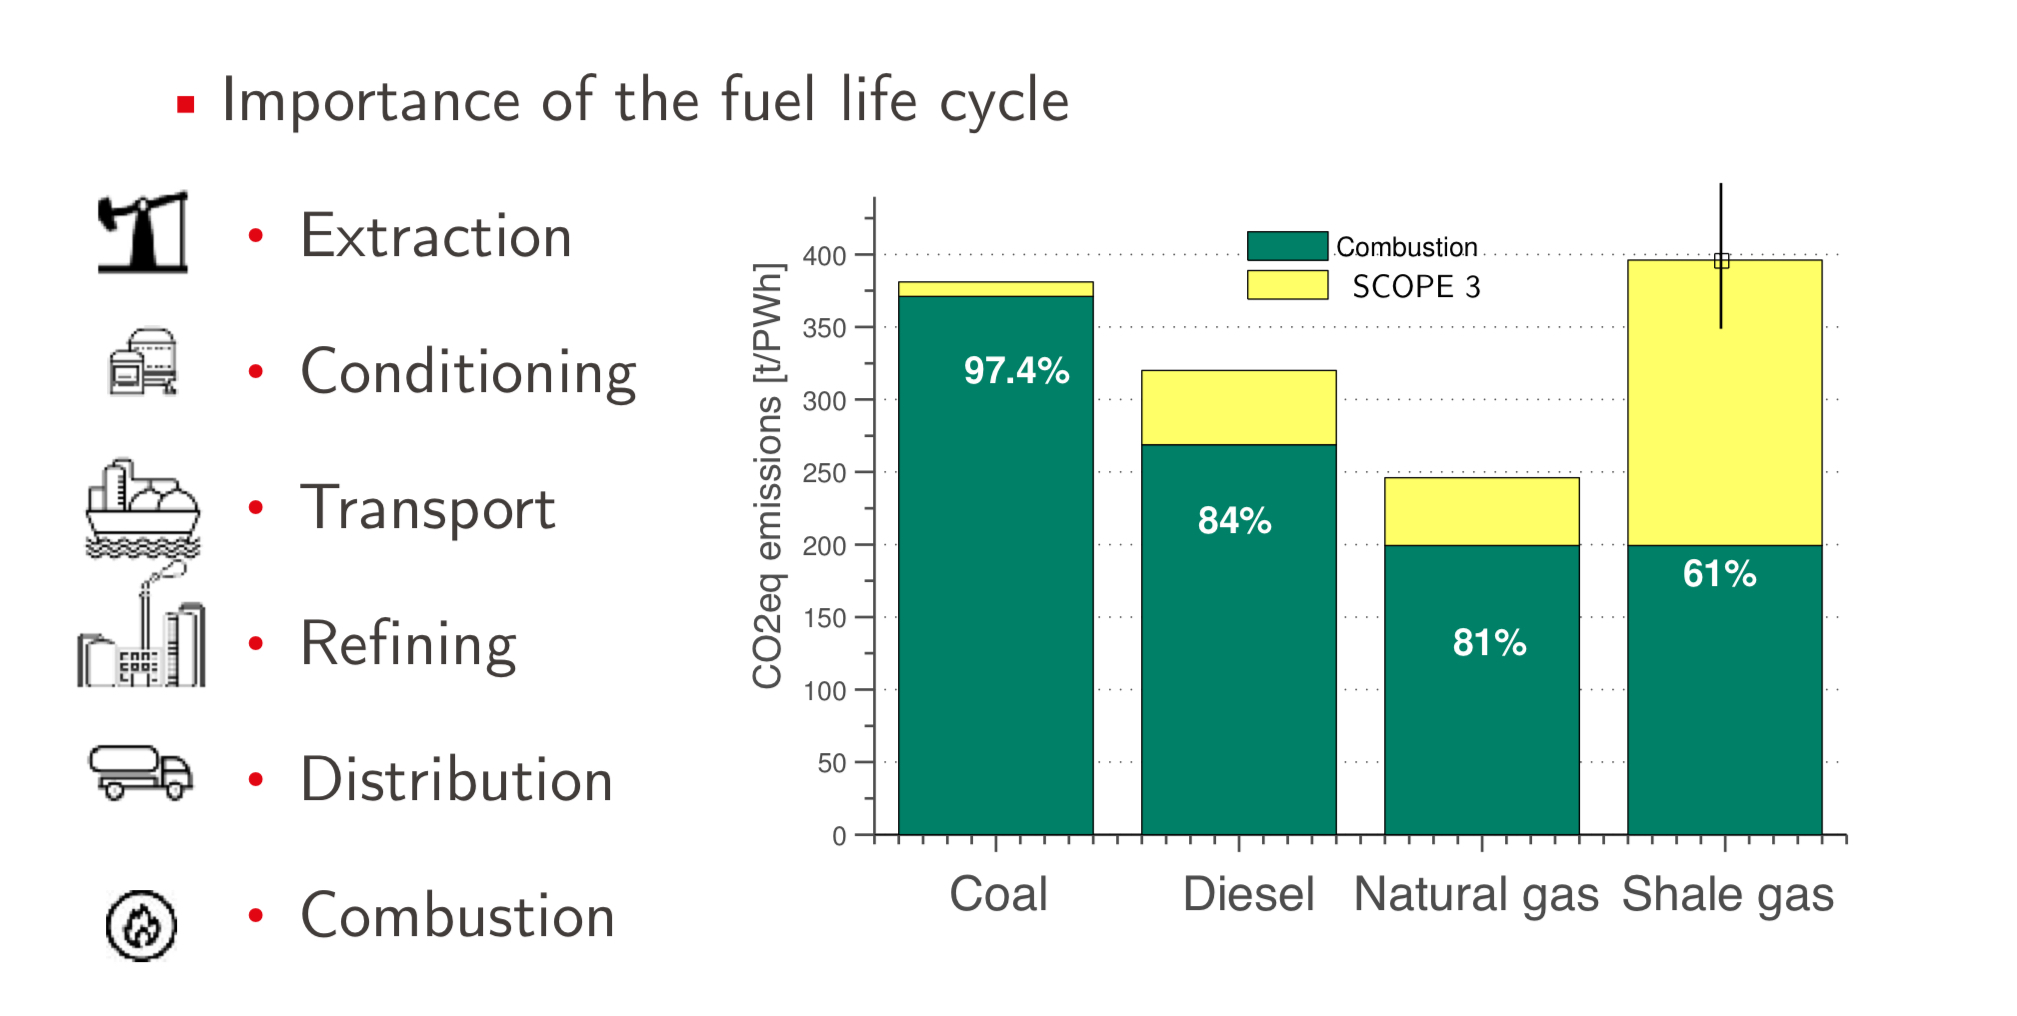
\includegraphics[width=0.8\linewidth]{IMAGES/LCA/IMG_0181.jpeg}
\end{figure}

Actions to mitigate the emissions : \begin{itemize}
    \item Measure 1 : flaring of off-gases
    \item Measure 2 : green completion, send back
    \item Measure 3 : tracking fugitive emissions
\end{itemize}

By renovating buildings, we can save up to $40\%$ in consumption. \\

The COP or coefficient of Performance is described as : \begin{equation}
    COP = \frac{\text{useful heat}}{\text{electricity}} \simeq 3
\end{equation}
It is close to 3 for heat pump.\\

Biomass electricity with $CO_2$ capture and sequestration: negative emissions. \\
\warning Impact is different if we consider different indicators. \\

\subsubsection{Harvesting renewable energy sources}

The energy return on energy invested is : \begin{equation}
    EROI = \frac{\text{electricity produced}}{\text{energy for panel production}}
\end{equation}

Smart renewable energy : impact from the system design (harvesting, efficiency, conversion), impact from the operation (costs vs $CO_2$ content vs Life Cycle Impacts), impact from the mix grid (25 years life time perspective).\\

\subsubsection{Integrating personal mobility}
The choice between EV and internal combustion car depends on the use we have. \\
A mix with PV panels and EV reduces by much the total emissions of a household.\\
In future, humans will need more energy to run data centers than the energy needed for heating up the water. But we can then use the heat generated by the data center to heat up the water.\\

The best that we can do would be to have an EV with PV panels, a data center and a heat pump in buildings.\\
From water waste, we can extract the methane and store it to use it for winter time when it can then be used with a fuel cell to generate electricity. For this, we need $25 m^2 PV/hab$ and cost about $12.5 k$\texteuro$/100m^2$ and is $100\%$ autonomous.\\

\subsection{Inventory}

\begin{theorem}
    Phase of life cycle assessment involving the compilation and quantification of inputs and outputs for a product throughout its life cycle.
\end{theorem}

\quad \underline{General procedure :}\\
\begin{enumerate}
    \item Obtain data for each unit process of the product-system (scaled to one product unit)
    \item Scale the intermediary flows to the functional unit (RF : quantity of products necessary to complete the function as expressed by functional unit)
    \item Scale the elementary flows to each of the unit processes to the functional unit
    \item Sum all the elementary flows on the entire life cycle
\end{enumerate}

\begin{figure}[hbt!]
    \centering
    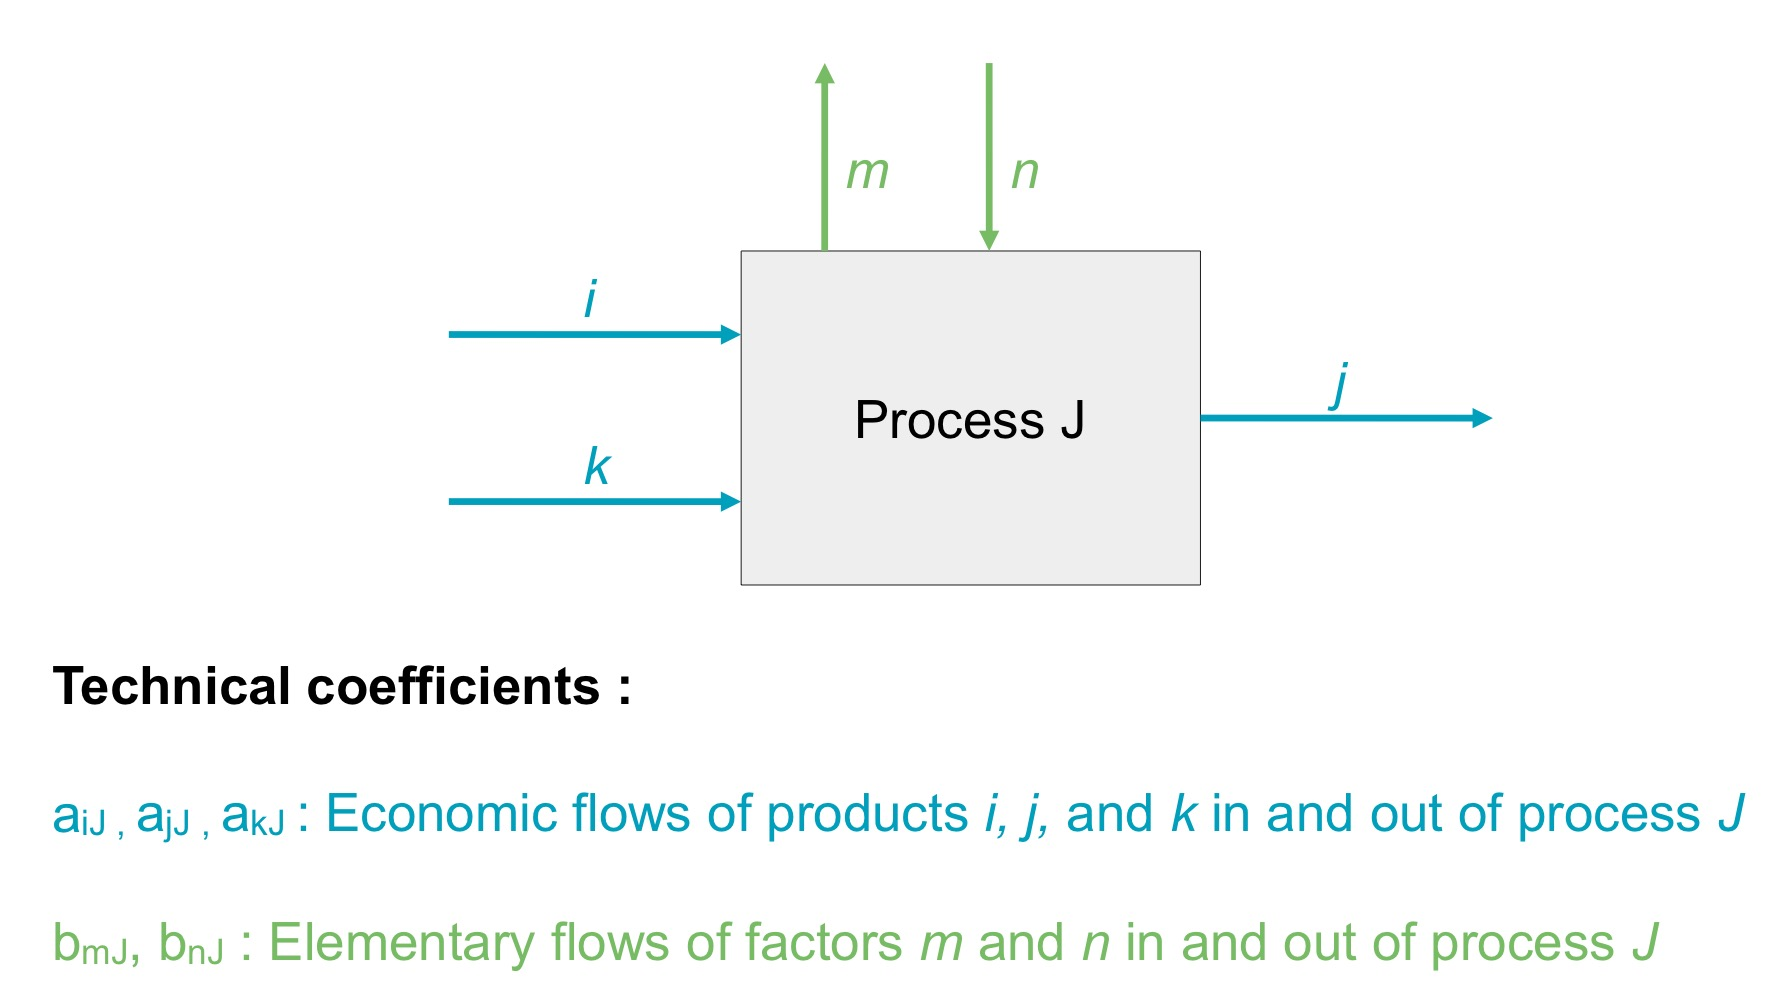
\includegraphics[width=0.6\linewidth]{IMAGES/LCA/IMG_0185.jpeg}
\end{figure}
By convention, positive for output and negative for inputs.\\

There exists two methods to solve : sequential method (set of rules of three, starting from the elementary process providing the FU and moving up the process tree) and matrix method (relies on a balance of intermediary flows).\\

\begin{itemize}
    \item Sequential method : we put each unit process to scale, one at a time starting from the process giving the function defined by the functional unit and by going up the process tree. It is simple and intuitive but the supply chains in the product systems are infinite (feedback loops). Only offers approximate solution
    \item Matrix method : a unit process could be represented by an elementary process vector $(p)$ with two components : intermediary flows $(a)$ and elementary flows $(b)$. The unit process vectors could be assembled in a matrix of elementary processes P that has two parts : \begin{itemize}
        \item Technology matrix A, exchanges between intermediary flows
        \item elementary flow matrix B, elementary flows for each process
        \begin{equation}
            \begin{gathered}
                A = \begin{pmatrix}
                    & p_1 & \cdots & p_n\\
                    p_1 & & \\
                    \vdots & & \\
                    p_n & & \\
                \end{pmatrix}, \:
                B = \begin{pmatrix}
                    & p_1 & \cdots & p_n\\
                    NG & & \\
                    \vdots & & \\
                    CO_2 & & \\
                \end{pmatrix}
            \end{gathered}
        \end{equation}
    \end{itemize}
    We then get the equation $As = f$ where $s$ represents the scaling factors and $f_i \neq 0$ only if it represents the function of the study. $Bs = g$ where $g$ are the elementary flows scaled and aggregated by the type of flow. \warning A is square and non-singular.

    It provides an exact solution.
\end{itemize}

\subsubsection{Inventory databases}
We can use a life cycle inventory database (LCI-DB) to generate the background of the LCA. 

Three different ways to build a LCI : \begin{enumerate}
    \item US LCI : the work of linking the unit processes together is done by analysts. No link between blocks
    \item Disaggregated : links between the processes are coded, meaning that the LCI calculations are done in the software
    \item Aggregated : pre-calculated datasets (no information on what is inside), allows for hiding confidential information and calculations are simpler.
\end{enumerate}

There is two types of LCA : \begin{itemize}
    \item Attributional : in case of a new requirement in electricity i.e., the share that plants provide to the network will be reevaluated
    \item Consequential : all cause and effect relationships could be considered. In this case, the new factory will not re-assess the entire grid but rather only use electricity from a plant that can provide it.
\end{itemize}

\subsection{Multifunctional processes}
When a process provides more than one function, we need to distribute the inputs and outputs to each of the functions to avoid double-counting.\\
\begin{enumerate}
    \item Avoid allocation as much as possible : 
    \begin{itemize}
        \item Divide the process in sub-processes
        \item Expand the system boundary of the product system (substract the alternative way of product B)
    \end{itemize}
    \item Allocate the inputs and outputs in a way that reflects underlying physical relationships existing between them (allocate resources according to their percentage in the output)
    \item Allocate inputs and outputs in a way that reflects other mutual relationships (mass, economic, $\cdots$).
\end{enumerate}

\begin{figure}[hbt!]
    \centering
    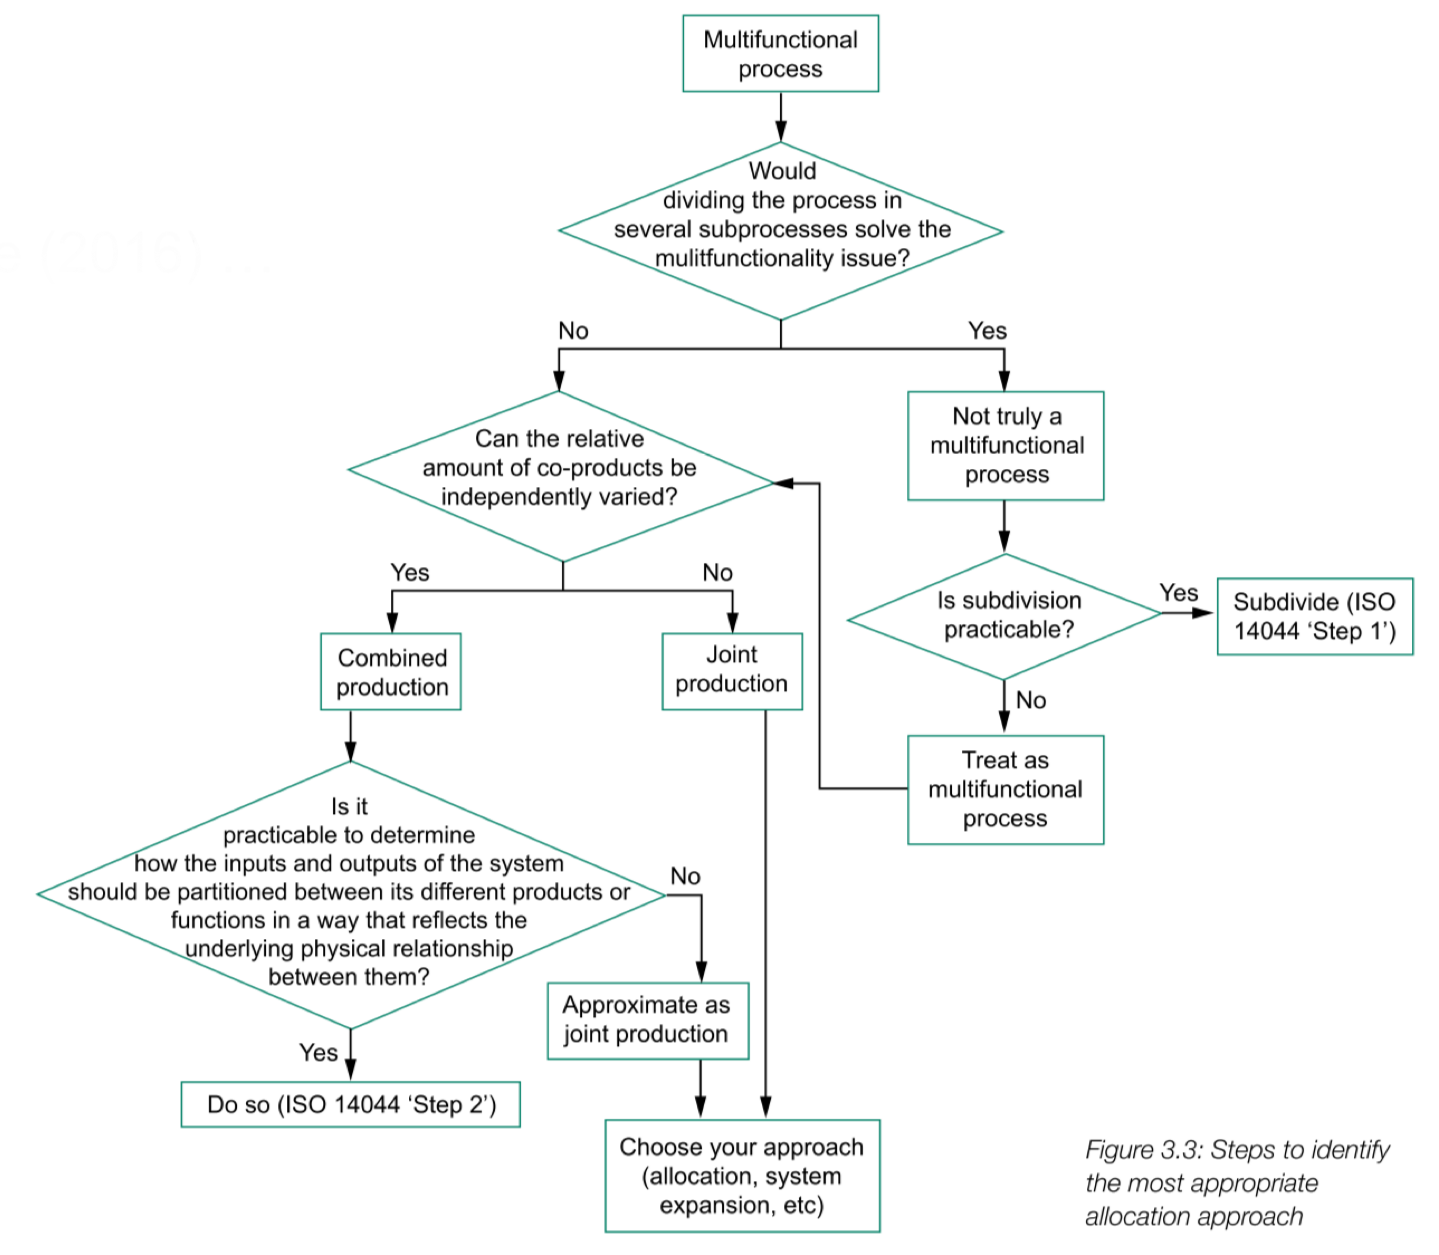
\includegraphics[width=0.8\linewidth]{IMAGES/LCA/Screenshot 2024-10-29 at 16.59.24.jpeg.png}
\end{figure}

\subsubsection{Recycling}
Open-loop recycling has two functions, each associated to its respective product system.\\
A product is manufactured from $x\%$ of virgin material and $y \%$ of recycled material. At the end of its life, $\alpha \%$ of the collected material goes to final disposal and $\beta \%$ is recycled.\\
Main approaches : \begin{itemize}
    \item Recycled content : Recycling is attributed to the life cycle that uses the recycled material. Recycling at the end of life is simply excluded from the system (no credits but no impact on EOL)
    \item End of life recycling : materials used in the life cycle are assumed as $100\%$ virgin regardless of the recycled content (assumed $0\%$). Recycling at the EOL avoids producing raw materials.
\end{itemize}

\subsection{Life cycle impact assessment (LCIA)}
Goal of an LCA : support decision-making. The inventory is not a good tool when too much elements are present.\\
Evaluated impacts scores only represent potential impacts (not real impacts, nor surpassing norms or risks). Due to : \begin{itemize}
    \item the relative expression of impacts in relation to a unit of reference
    \item the integration of inventory data over space and time
    \item the inherent uncertainty in modeling impacts and the lack of information about the specific conditions of the exposed environment
    \item the fact that some impact categories clearly suggest future impacts
\end{itemize}

To compare substances/resources we need to find comparison criteria.\\
Cause-effect chain : \begin{itemize}
    \item encompass a series of environmental mechanisms
    \item each impact category has its own environmental mechanism 
    \item domino effect that allows to map the pathways that link the LCI to the category indicators of an impact category
\end{itemize}
Midpoints are expressed in $kg_{CO2-eq}$ while the damages are expressed in global units. \\
The LCI can be expressed with midpoints and finally in damages.\\
A characterization factor (CF) represents the potential impact per quantity of an elementary flow to a given impact category.\\

\begin{figure}[hbt!]
    \centering
    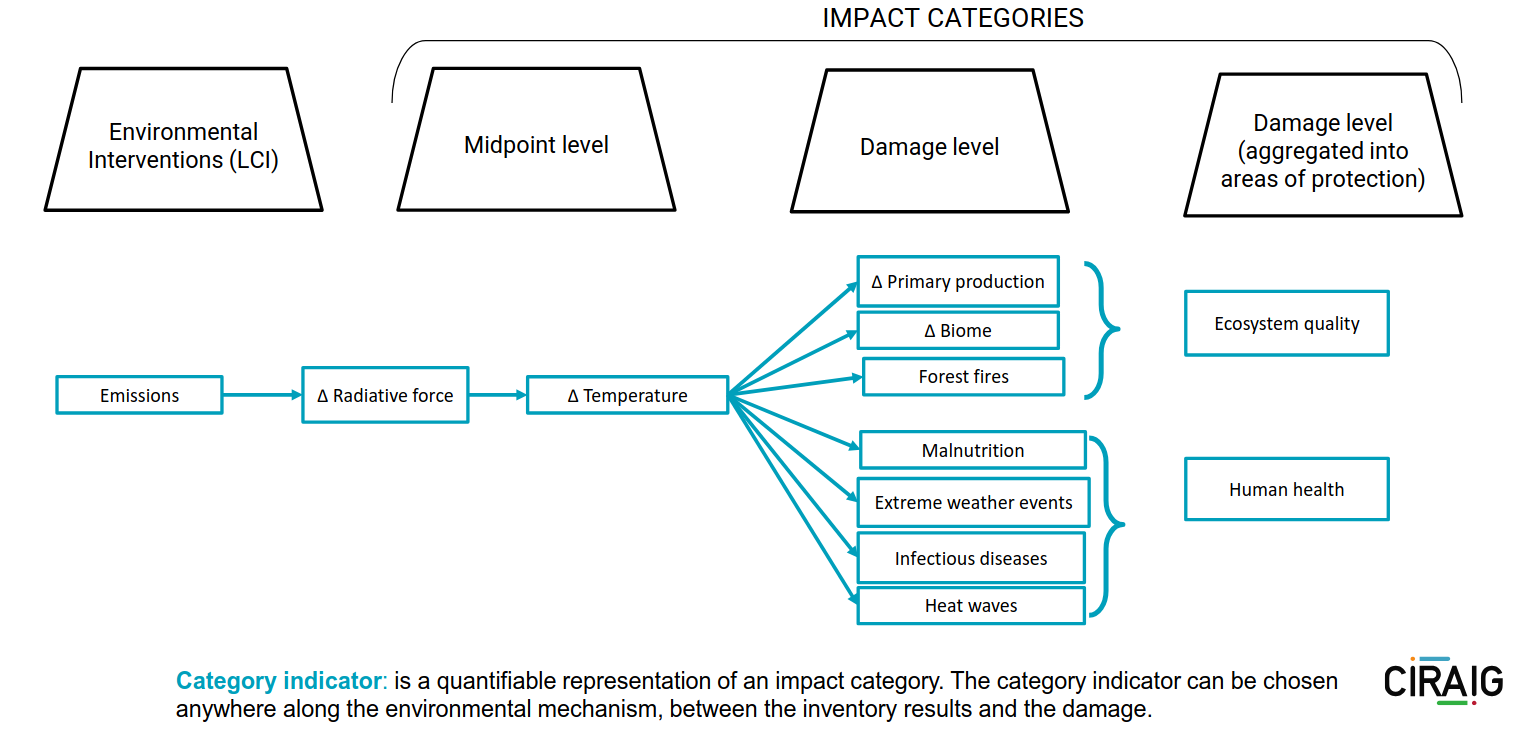
\includegraphics[width=0.7\linewidth]{IMAGES/LCA/Screenshot from 2024-11-12 17-24-00.png}
\end{figure}

An impact indicator is a quantified representation of an environmental issue. The midpoint indicator can be chosen anywhere along the environmental mechanism, between the inventory and the damages.\\
Moving down the causality chain we are increasing environmental relevance, decreasing uncertainty of interpretation and increasing uncertainty from characterization models.\\

Make sure that the choices reflect a complete set of environmental problems related to the studied product system. The impact categories are not redundant and in some cases new impact categories have to be defined.\\
An emitted substance could contribute to many potential impacts.\\
*The impact score per category is then simply : $h_i = \sum CF_{ji} g_i$ with $CF_{ji}$ the characterization factor of the elementary flow i for the impact category j and $g_i$ the elementary flow ($kg_i$).\\
The mandatory elements are then : \begin{enumerate}
    \item Selection of impact categories, category indicators and characterization models
    \item Assignment of LCI results (classification)
    \item Calculation of category indicator results (characterization)
\end{enumerate}

Aggregation of damage indicators within 3 areas of protection : \begin{itemize}
    \item DALY : "disability adjusted life years", number of years (in good health) lost, premature mortality or a certain degree of illness for a certain time
    \item $PDF \cdot m^2 \cdot yr$, "potential of disappeared fraction of species", percentage of species disappeared over a certain surface over a certain amount of time
    \item $\$$, potential costs that society has to bear to maintain or replace the same service
\end{itemize}


We now have some optional elements : \begin{enumerate}
    \item Normalization
    \item Weighting
    \item Aggregation
\end{enumerate}

This is done to compare the impacts of a scenario with the impact of a reference system and put the results in perspective.\\
The normalization can be external (the reference is the total impact of an external system such as a country) or internal. \\
In order to obtain one single score, one should use weighting factor to compare damages. \\

\warning Weighting and aggregation are not permitted for LCA used to support public comparative assertion!\\

Principles of weighting : \begin{itemize}
    \item Monetization
    \item Expert panel (evaluation by expert)
    \item Distance to target 
\end{itemize}

The grouping method relies on the sorting and ranking in order of priority of the impact categories. 
The life cycle impact is then : \begin{equation}
    h =cg = cBs= cBA^{-1}f
\end{equation}
with h the life cycle impact score vector, c the matrix including the characterization factor of each impact. \\
LCIA cannot always demonstrate significant differences in results as we have \begin{itemize}
    \item limited coverage of relevant impact categories
    \item limited development of characterization models, sensitivity analysis and uncertainty analysis
    \item no characterization factors for all reference flows
\end{itemize}

\subsection{LCA interpretation fundamentals}
Framework : \begin{enumerate}
    \item Identification of significant points
    \item Verification (sensitivity analysis, $\cdots$)
    \item Conclusions, recommendations
\end{enumerate}

Theoretical structure of LCIA models : Emission $\Rightarrow_{FF}$ Receiving media $\Rightarrow_{XF}$ Exposure $\Rightarrow_{EF}$ Effect. With FF the fate factor (distribution of a contaminant emitted in a compartment into receiving compartments at steady state), XF the exposure factors (fraction of the contaminant in each receiving compartment that reach the subject of safeguard via different exposition pathways at steady state), EF the effect factors (quantity of adverse effects per quantity of exposure to the contaminant).\\

\subsubsection{Interpretations of LCA results}
Structure the results from the LCI and LCIA phases in order to help determine the significant issues. \\

\begin{figure}[hbt!]
    \centering
    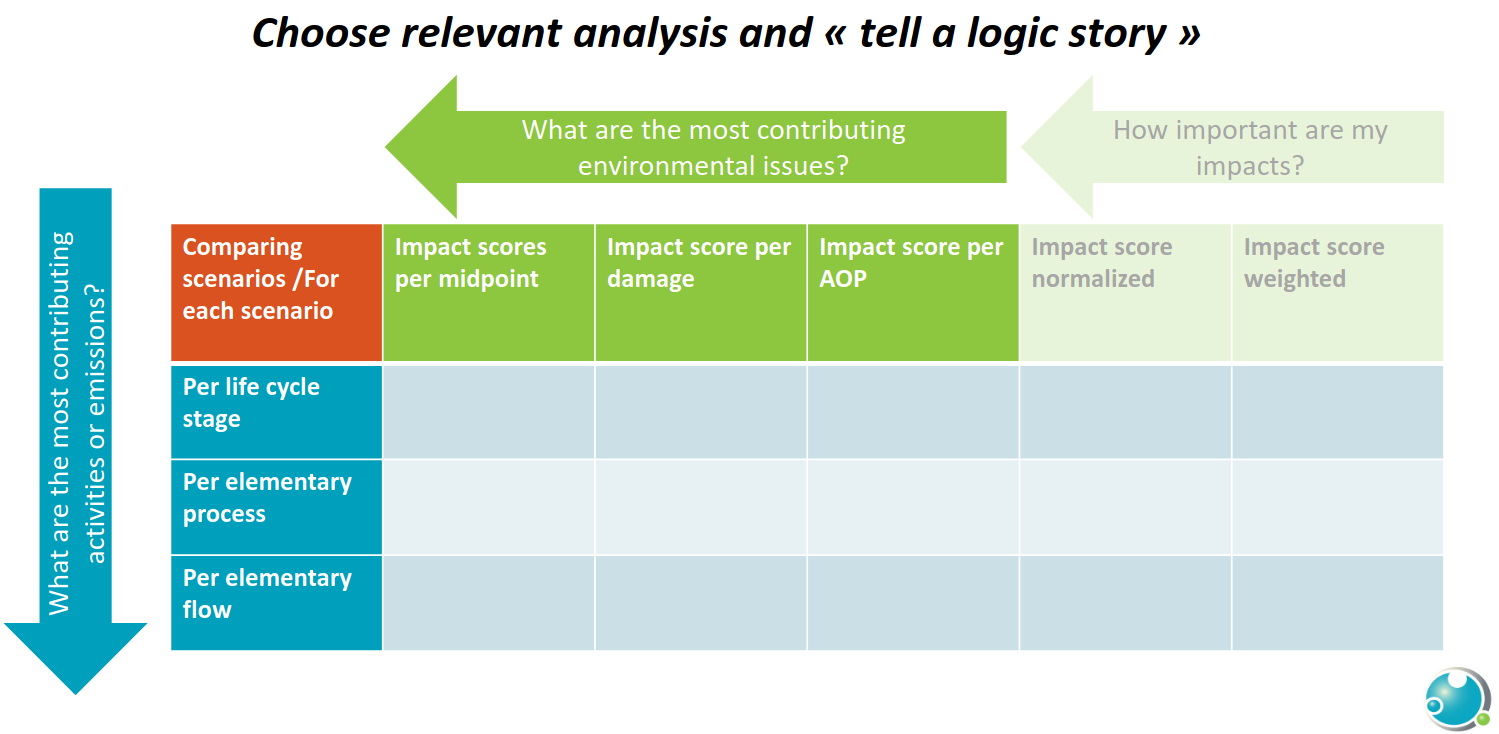
\includegraphics[width=0.8\linewidth]{IMAGES/LCA/Screenshot from 2024-11-19 16-42-24.png}
\end{figure}

Other methods to identify significant points : \begin{itemize}
    \item Dominance analysis : by using statistical tools or other techniques such as qualitative or quantitative ranking, significant or outstanding contributions are studied
    \item Influence analysis : ability to influence an environmental aspect is examined
    \item Evaluation of misstatements : surprising or unusual deviations are identified
\end{itemize}

\subsubsection{Verification}
Establish and enhance confidence and the reliability of the results of the LCA study, including the significant issues identified.\\
Three steps : \begin{itemize}
    \item Sensitivity analysis : estimate the effects of the choices made regarding methods and data on the outcome of a study
    \item Control of completeness : ensure that relevant information and data required for the interpretation are available and complete
    \item Control of consistency : determine wether the assumptions, methods and data are consistent with the purpose and scope of the study
\end{itemize}
Put your effort on improving data collection where it is sensitive! 

\warning Methodology such as ReCiPe assume that the LCA has be made using European data, TRACI uses USA data and LIME uses japanese data.


\end{document}